\section{D -- AtCoDeer and Rock-Paper}

\begin{frame}[fragile]{Problema}

AtCoDeer the deer and his friend TopCoDeer is playing a game. The game consists of $N$ turns. In
each turn, each player plays one of the two gestures, Rock and Paper, as in Rock-paper-scissors,
under the following condition:

\vspace{0.1in}

(*) After each turn, (the number of times the player has played Paper) $\leq$ (the number of times
the player has played Rock).

\vspace{0.1in}

Each player's score is calculated by (the number of turns where the player wins) - (the number of
turns where the player loses), where the outcome of each turn is determined by the rules of
Rock-paper-scissors.

\end{frame}


\begin{frame}[fragile]{Problema}



\end{frame}

\begin{frame}[fragile]{Entrada e saída}

\textbf{Constraints}

\begin{itemize}
    \item $3\leq H\leq 10^9$
    \item $3\leq W\leq 10^9$
    \item $0\leq N\leq \min(10^5, H\times W)$
    \item $1\leq a_i\leq H\ (1\leq i\leq N)$
    \item $1\leq b_i\leq W\ (1\leq i\leq N)$
    \item $(a_i, b_i) \neq (a_j, b_j)\ (i\neq j)$
\end{itemize}

\end{frame}

\begin{frame}[fragile]{Entrada e saída}

\textbf{Input}

Input is given from Standard Input in the following format:
\begin{atcoderio}{llll}
$H$ & $W$ & $N$ \\
$a_1$ & $b_1$ \\
$\vdots$ \\
$a_N$ & $b_N$ \\
\end{atcoderio}

\vspace{0.1in}

\textbf{Output}

Print 10 lines. The ($j + 1$)-th ($0\leq j\leq 9$) line should contain the number of the
subrectangles of size $3\times 3$ of the grid that contains exactly $j$ black cells.

\end{frame}

\begin{frame}[fragile]{Exemplo de entradas e saídas}

\begin{minipage}[t]{0.55\textwidth}
\textbf{Entrada}
\begin{verbatim}
4 5 8
1 1
1 4
1 5
2 3
3 1
3 2
3 4
4 4
\end{verbatim}
\end{minipage}
\begin{minipage}[t]{0.4\textwidth}
\textbf{Saída}
\begin{verbatim}
0
0
0
2
4
0
0
0
0
0
\end{verbatim}
\end{minipage}
\end{frame}

\begin{frame}[fragile]{Exemplo de entradas e saídas}

    \begin{figure}
        \centering

        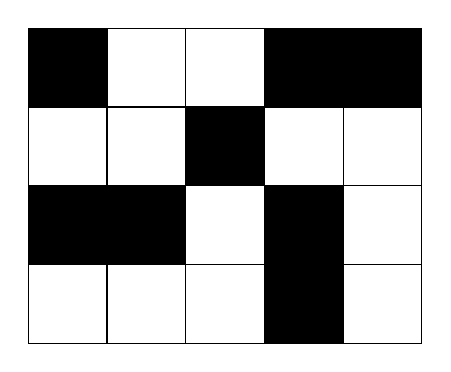
\begin{tikzpicture}
            \draw (0, 0) grid (5, 4);

            \fill[black] (0, 1) rectangle (2, 2);
            \fill[black] (0, 3) rectangle (1, 4);
            \fill[black] (2, 2) rectangle (3, 3);
            \fill[black] (3, 0) rectangle (4, 2);
            \fill[black] (3, 3) rectangle (5, 4);
        \end{tikzpicture}

    \end{figure}

\end{frame}


\begin{frame}[fragile]{Solução}

    \begin{itemize}
        \item Há um total de $(H - 2)(W - 2)$ quadrados $3\times 3$ a serem avaliados

        \item Como $H, W\leq 10^9$, a verificação individual de cada um destes quadrados leva a
            um veredito TLE

        \item Contudo, o número total de pontos pintados $N$ é menor ou igual a $10^5$

        \item Cada ponto pertence a um total de 9 destes quadrados

        \item Assim, é possível resolver o problema verificando, no máximo, $9\times 10^5$
            quadrados, pois todos os demais certamente não terão nenhum ponto pintado

    \end{itemize}

\end{frame}


\begin{frame}[fragile]{Solução}

    \begin{itemize}
        \item Considere que cada quadrado seja caracterizado pelo seu canto superior esquerdo

        \item Cada ponto pintado $(x, y)$ pertence a um dos 9 quadrados cujo canto superior
            esquerdo tem coordenadas $(x - d_x, y - d_y)$, com $0\leq d_x, d_y\leq 2$

        \item Um dicionário deve registrar, para cada possível canto superior esquerdo, quantos
            pontos pintados fazem parte de seu quadrado associado

        \item Deve-se atentar que o número de quadrados sem nenhum ponto pintado é a diferença
            entre o total e os que tem ao menos um ponto pintado

        \item Esta soluçã tem complexidade $O(N\log N)$
    \end{itemize}

\end{frame}

\begin{frame}[fragile]{Solução $O(N\log N)$}
    \inputsnippet{cpp}{1}{20}{codes/D.cpp}
\end{frame}

\begin{frame}[fragile]{Solução $O(N\log N)$}
    \inputsnippet{cpp}{21}{40}{codes/D.cpp}
\end{frame}

\begin{frame}[fragile]{Solução $O(N\log N)$}
    \inputsnippet{cpp}{41}{60}{codes/D.cpp}
\end{frame}
